\documentclass[a4paper,10pt]{article}

% Packages
\usepackage[utf8]{inputenc}
\usepackage[T1]{fontenc}
\usepackage[margin=1.5cm]{geometry}
\usepackage{paracol}
\usepackage{graphicx}
\usepackage{setspace}
\usepackage{enumitem}
\usepackage{titlesec}
\usepackage{tabularx}
\usepackage{tikz}
\usepackage[most]{tcolorbox}

% Fonts ---
\usepackage{fontspec}
\setmainfont{Roboto} % Change to your preferred font


\newfontfamily\ubuntu[
    Path = ../fonts/,
    UprightFont = Ubuntu-Regular.ttf,
    BoldFont    = Ubuntu-Bold.ttf,
    ItalicFont  = Ubuntu-Italic.ttf,
    BoldItalicFont = Ubuntu-BoldItalic.ttf
]{Ubuntu}
% Fonts ---

% Section title style (uppercase, spaced)
\titleformat{\section}{\bfseries\uppercase}{\thesection}{0.5em}{}

% No numbering
\setcounter{secnumdepth}{0}

% Reduce space between items
\setlist[itemize]{nosep,left=0pt}

\begin{document}
% --- Side 1 starter her fra ---

% Header
\noindent CV / \textbf{Elias Elfarri} \hfill \textbf{Mobil utvikler} \\
\rule{\linewidth}{0.5pt}


% Space before header
\vspace{3em}

\begin{paracol}{2}
% ----- Left column -----
\begin{flushleft}
    % Profile picture
    \begin{tikzpicture}
     \clip (0,1.5) circle (2cm); % adjust size (radius)
     \node at (0,0) {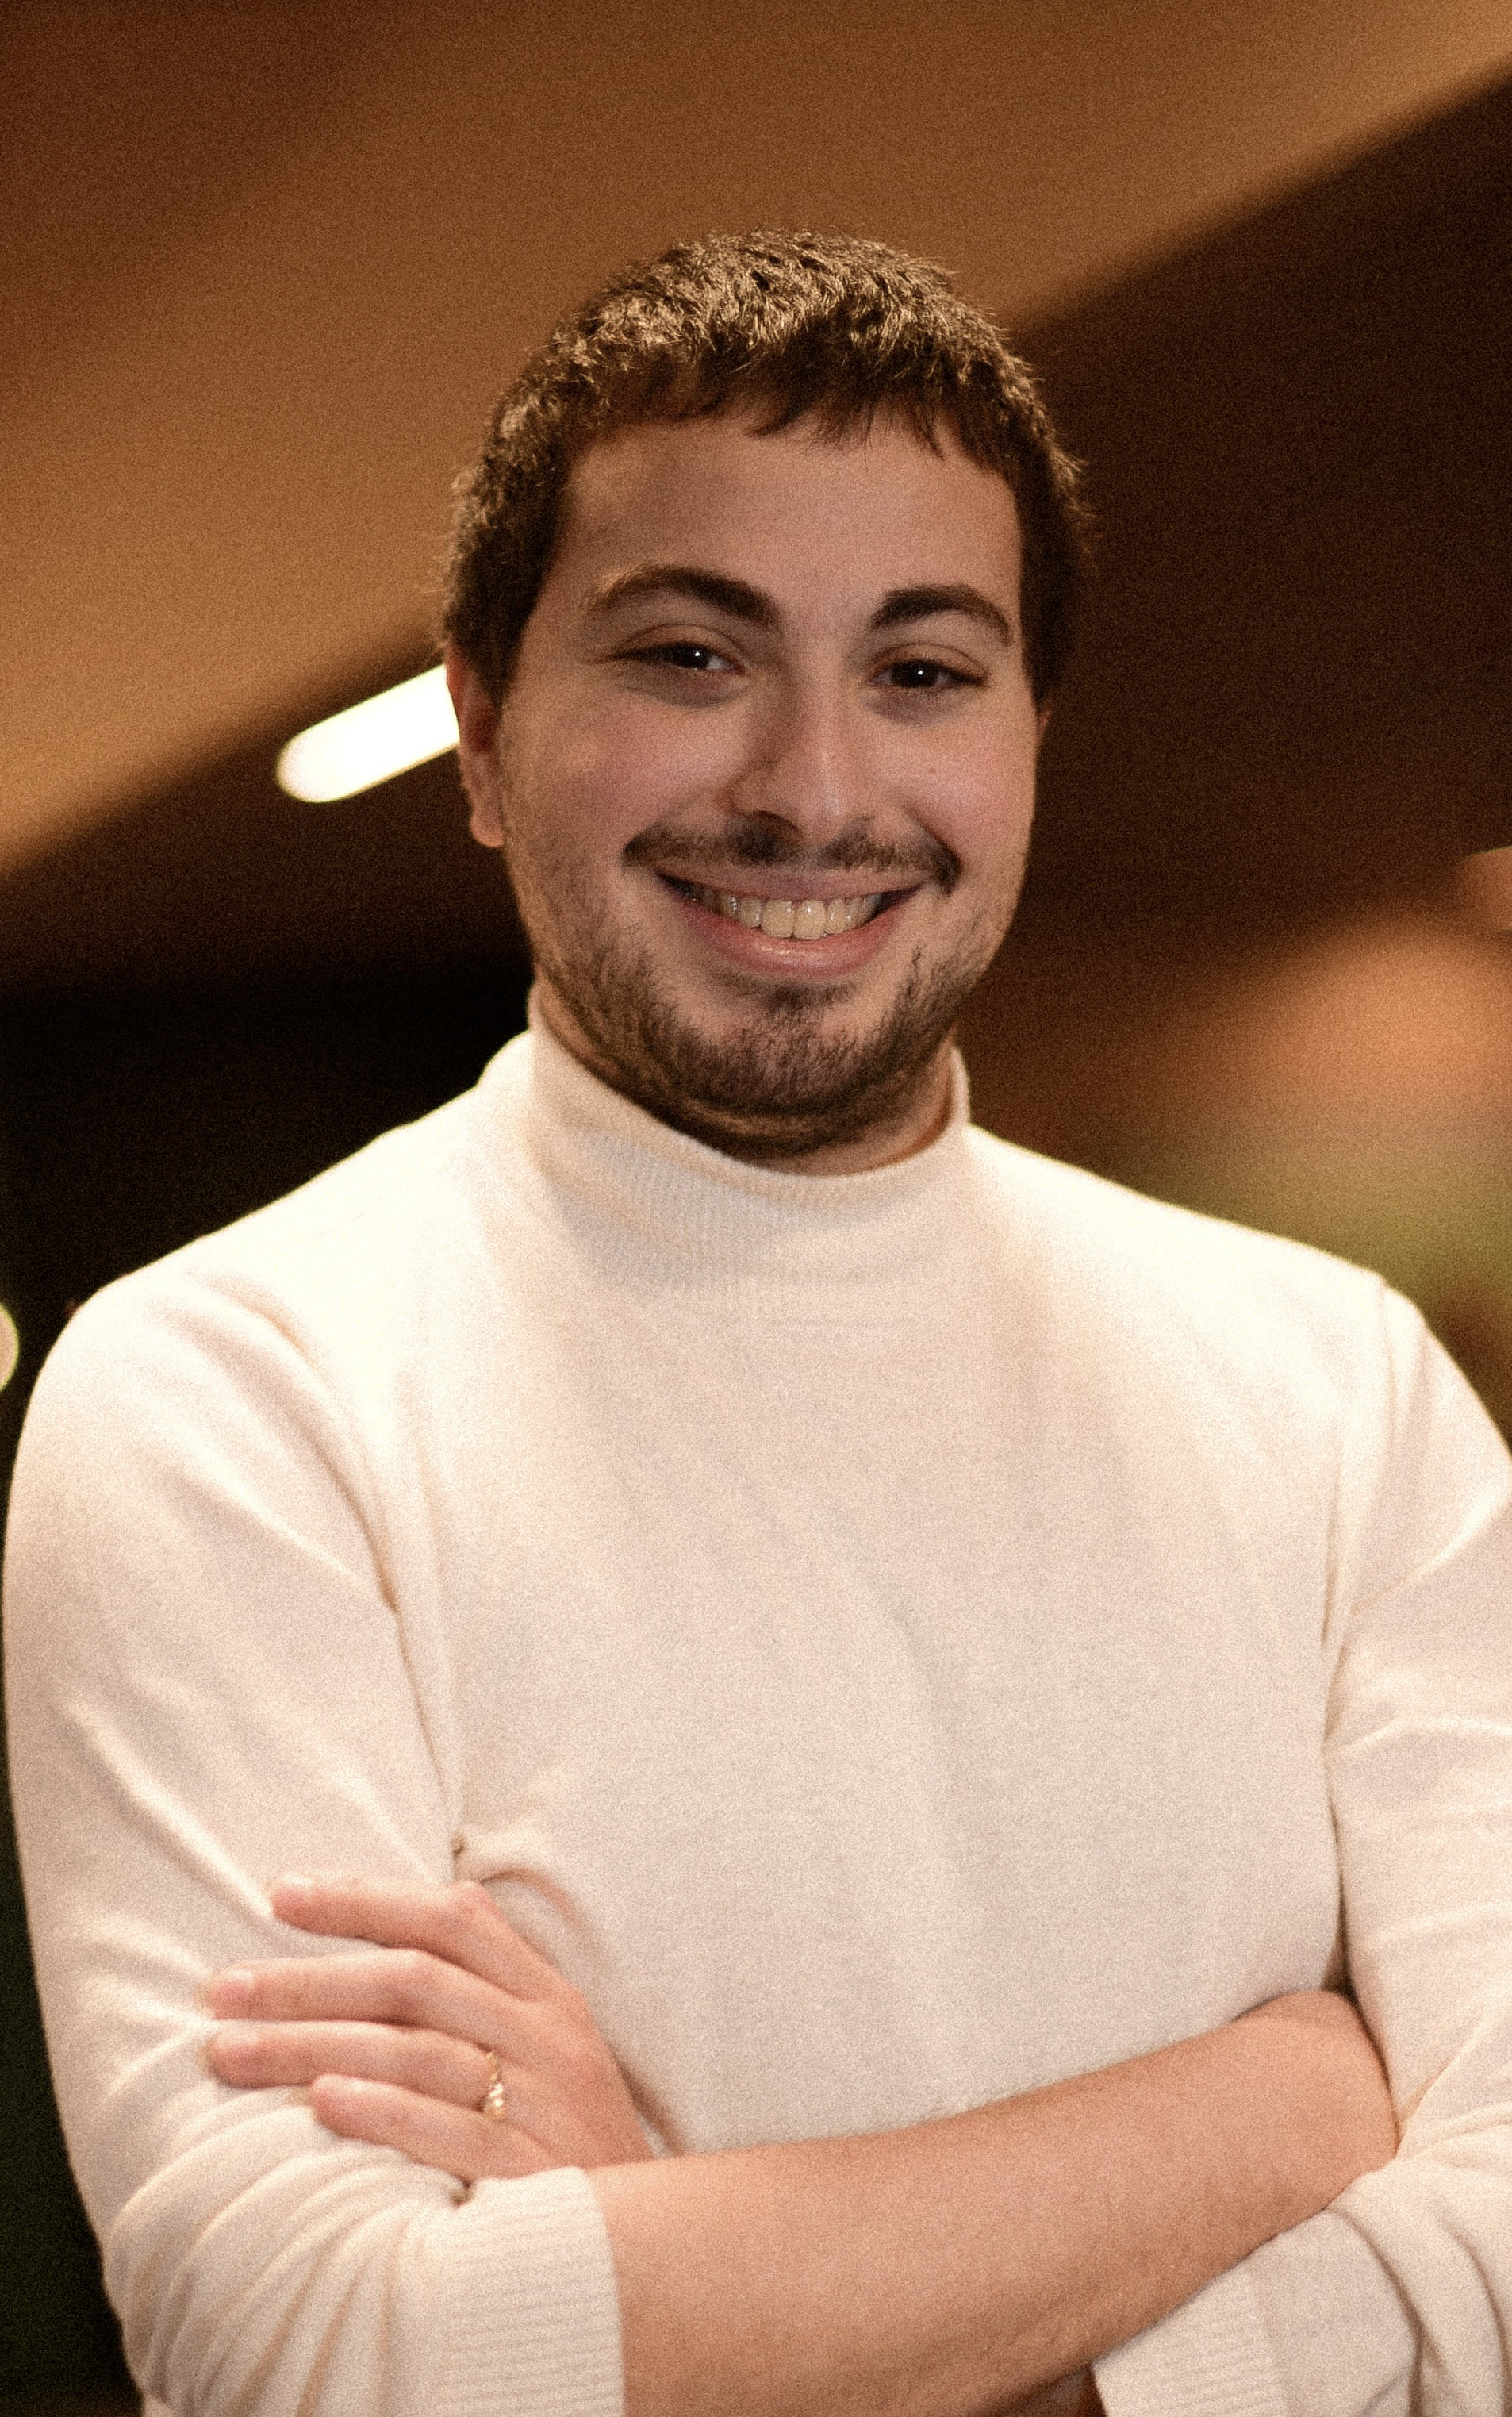
\includegraphics[width=5cm]{../portrait.jpg}};
    \end{tikzpicture}

    % a bar between image and name
    \vspace{1em}
    \noindent\rule{4cm}{10pt}
    

    \vspace{1.5em}
    {\Huge \ubuntu{Elias Elfarri}} \\
    \vspace{0.5em}
    
    \begin{tcolorbox}[
        colback=white,       % background color
        colframe=white,      % border color
        boxrule=0.0pt,       % border thickness
        arc=2mm,             % rounded corners
        width=0.85\linewidth,% make box narrower than column
        left=0mm, right=2mm, top=1mm, bottom=1mm % inner padding
        ]
    
    Elias er en mobilutvikler med 
    fire års erfaring fra både native-utvikling
     i Swift og Kotlin og kryssplattform med Flutter/Dart.
      Han har bygget opp mobilteam,
       ledet utviklingen av skalerbare
        kodebaser og publisert syv apper 
        på App Store og Google Play. 
        Med erfaring som spenner fra BLE,
         kamera og sanntids grafer til widgets 
         og spesialisert hardware-integrasjon,
          behersker han hele spekteret av
           mobilutvikling.
      Han er kjent som initiativrik, 
      reflektert og har gode pedagogiske evner.
       Elias leder Flutter Meetup-nettverket i 
       Oslo/Norge med over 500 medlemmer,
        hvor han arrangerer samlinger, 
        kurs og hackathons. 
        Dette engasjementet 
        gjør ham til en pådriver som både løfter
         prosjekter og kolleger.
    \end{tcolorbox}
\end{flushleft}

\switchcolumn

\vspace{5em}
\begin{center}
    
\end{center}
\vspace{2em}

% ----- Right column -----
 
\section{\ubuntu ERFARING}
\renewcommand{\arraystretch}{1.3} % Spacing between rows
\begin{tabularx}{\columnwidth}{@{}lX@{}}
2022 -- d.d & Fink AS, Mobil utvikler \\
2023 -- 2025 & Fink AS, Fagansvarlig Mobilutvikling \\
2021 -- 2022 & DNV, Frontend utvikler \\
2019 -- 2020 & Jenteprosjektet Ada, Prosjekt assistent \\
2018 -- 2022 & SIT, Team leder \\
2017 -- 2018 & NVFT AS, Promotør \\
2015 -- 2016 & Oslo Kommune, Hjelpepleier \\
\end{tabularx}

% space and line
\vspace{0.5em} 
\noindent\rule{\linewidth}{0.2pt}

\section{\ubuntu Utdanning}
\renewcommand{\arraystretch}{1.3} % Spacing between rows
\begin{tabularx}{\columnwidth}{@{}l>{\raggedright\arraybackslash}X@{}}
2017 -- 2022 & Norges teknisk-naturvitenskapelige universitet, Master i kybernetikk og robotikk, Sivilingeniør \\
2017 -- 2017 & Université de Caen Normandie, Utveksling \\
2016 -- 2017 & Norges teknisk-naturvitenskapelige universitet, Årsstudium i Fransk språk og litteratur \\
\end{tabularx}

% space and line
\vspace{0.5em} 
\noindent\rule{\linewidth}{0.2pt}


\section{\ubuntu Kunder}
DNV, \hspace{0.1em} 
InlineX, \hspace{0.1em} 
Norges teknisk-naturvitenskapelige
universitet

% space and line
\vspace{0.5em} 
\noindent\rule{\linewidth}{0.2pt}

\section{\ubuntu Roller}
Tech lead, \hspace{0.1em}
Mobil utvikler, \hspace{0.1em}
Frontend utvikler, \hspace{0.1em}
Fagansvarlig

\end{paracol}

\vfill
\noindent\rule{\linewidth}{0.5pt}\\
\hfill 

\newpage
% --- Side 2 starter her fra ---
% Header
\noindent CV / \textbf{Elias Elfarri} \hfill \textbf{Mobil utvikler} \\
\rule{\linewidth}{0.5pt}

  

 % TODO: add erfaringer inlinex: 2022, 2023, 2024, 2025, 2026
 % TODO: add erfaringer fra hva jeg gjorde i masteren 
 % TODO: Add Seksjon med publikasjoner, foredrag, leserinnlegg
 % TODO: Legg til tlf nr og email i headeren på første side
 % --- Verv seksjon ---
\section{Verv}
\begin{tabularx}{\linewidth}{@{}lX@{}}
2023 -- d.d & Flutter Oslo Meetup gruppe, Arrangør og leder \\
2024 -- d.d & Flutter and Friends Conference Stockholm, Arrangør \\
2018 -- 2019 & ISFiT, Dialog koordinator \\
\end{tabularx}
\vspace{1em}

% --- Stor tittel for prosjekter ---
\section{{\Huge \ubuntu PROSJEKTER}}

% --- Erfaring ---
\noindent
\begin{tabular}{@{}p{4cm}p{11cm}@{}}  % venstre = bredere, høyre = beskrivelse
\textbf{InlineX} & \textbf{Prosjekt:} I utgangspunket et prosjekt som skulle handle om at jeg skulle lage en mobil app hasteløsning som skulle dekke behovet for kunder uten internett, ble mye mer enn det. Startupen jeg kom inn i hadde lite kompetanse innenfor å jobbe med software til å være et selskap som drev med produktutvikling. Så dette ble starten på min reise som mobil utvikler og veldig formativt i forhold til å etterhvert bli ekstremt viktig kjernekompetanse for bedriften og etablere meg som techlead. Når jeg begynte hadde vi et skeleton crew, startupen var totalt på 6 stykk når jeg kom inn og de hadde meg på mobilutvikling og en til på webutvikling. Den største utfordringen med dette prosjektet var ikke den tekniske utførelsen av appen, men heller at de hadde ingen teknisk infrastruktur, ingen design, ingen produktavdeling, rett og slett ingenting på plass. Det tok litt tid å bygge opp dette fra bunnen, og denne erfaringen var nok bare starten på en langstrakt kamp om å forme selskapets produktavdeling til å bli skikkelig bra.   \\
& \\
& \textbf{Kompetanser:}  \\
\end{tabular}


 
\vspace{2em}

% --- Erfaring ---
\noindent
\begin{tabular}{@{}p{4cm}p{11cm}@{}}  % venstre = bredere, høyre = beskrivelse
\textbf{DNV} & \textbf{Prosjekt:} Elias har utviklet nye funksjoner i DP-CAP og DYN-CAP \\
Maritime Cybernetics Advisory & applikasjonene, brukt til beregninger og sertifisering av dynamisk posisjonering av skip. Han utviklet i Python/OpenCV basert på\\
2021 -- 2022 & Watershed-metoden, som reduserte manuelt arbeid fra flere dager til sekunder, og som ble kritisk for sertifiseringsanalyser bestilt av kunder som Equinor. Dette økte lønnsomheten av disse rapportene massivt, med en fastpris på 100 000 NOK så tok det et par klikk å levere samme analyse som kunne ta opp til en uke før. \\
& \\
& \textbf{Rolle:} Systemutvikler, backend, frontend, bildebehandlingsingeniør. \\
& \\
& \textbf{Kompetanser:} TypeScript, React, ClojureScript, Reframe, Clojure, Java, Python (OpenCV), bildebehandling/Computer Vision, PID-regulator, DP-posisjonering, Watershed algoritmen og klassisk bildebehandling. \\
\end{tabular}
 


\vfill
\noindent\rule{\linewidth}{0.5pt}\\
\hfill 

\end{document}